\xchapter{Methodology}{}

In this chapter, we present formulations to the many variants of the source code attribution problem in Section \ref{sec:formulations}, we describe how the Codeforces dataset was assembled in Section \ref{sec:dataset} and present a top-down approach to how the end-to-end model was developed in section \ref{sec:framework}.

\section{Problem Formulation}\label{sec:formulations}
\section{Datasets}\label{sec:dataset}

The first step to develop an effective deep learning model is to gather enough training data. In this work, we decided to work with C++ source codes written in a laboratory environment -- we assume the whole code is written by the author under no external style enforcement such as a style guide.

\subsection{Google Code Jam}

Although there are many public C++ laboratory datasets, the Google Code Jam\footnote{\url{https://codingcompetitions.withgoogle.com/codejam}} dataset \cite{caliskan_2015} is probably the biggest of them all. Samples from this dataset are collected from previous editions of Google Code Jam, an annual programming competition held by Google. In this competition, participants are given algorithmic tasks to be solved in a limited amount of time. As such, it's very likely that code written by a participant manifests his own coding style.

Google Code Jam holds nearly 10 rounds every year. Most of these rounds are eliminatory. Thus, the availability of samples from less experienced participants is expected to be low. If we want to build a balanced training set not biased by the way experienced participants code, we are limited by the small amount of code less experienced participants wrote.

Although this dataset was not extensively used throughout the development phase, it was a reference for the Codeforces dataset introduced in Section \ref{sec:codeforces}.

\subsection{Codeforces}\label{sec:codeforces}

Codeforces\footnote{\url{http://codeforces.com}} is a website specialized in holding online programming contests. Contest format is similar to Google Code Jam's, but they are not eliminatory. Thus, we are able to find a lot of samples from both non-experienced and experienced users.

We wrote a Python script that receives target constraints for the dataset and scrapes Codeforces for samples. Using this script, we assembled a balanced dataset with more than 30,000 samples from nearly 2,000 authors, meaning that we have around 15 samples per author. This dataset was packaged and made public\footnote{link-pro-dataset}.
% TODO: more details on filters
% TODO: add link to dataset

\section{Source Code Embedding Model}\label{sec:framework}

In this section, we propose a deep learning model that embeds source codes, from their string representations, into a denser latent space. In Section \ref{sec:descriptor}, we describe what is a style descriptor. In Section \ref{sec:models}, we describe network architectures used in our work. In Section \ref{sec:optimization}, we describe how our embedding network was trained to generate meaningful descriptors.

\begin{figure}[ht]
	\centering
	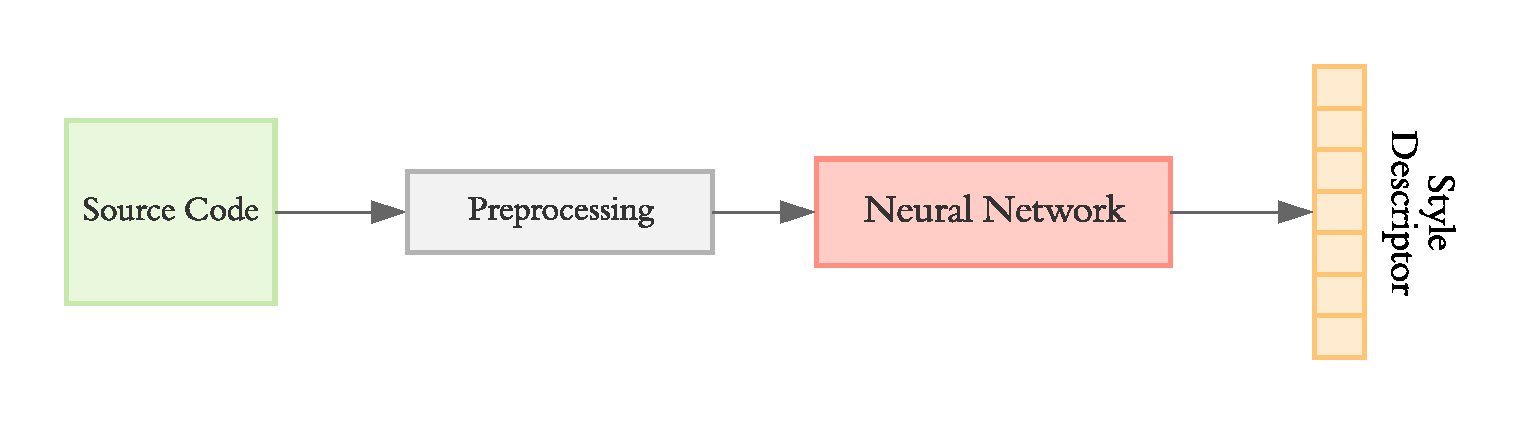
\includegraphics[width=\linewidth]{imgs/pipeline.pdf}
	\caption{Overview of style descriptor generation pipeline.}
	\label{fig:overall}
\end{figure}
% TODO: se referir a essa figura em algum lugar

\subsection{Coding Style Descriptor}\label{sec:descriptor}

The performance of machine learning methods is heavily affected by the choice of data representation. Thus, much of the effort of the machine learning community has been put into developing algorithms that transform otherwise unmanageable data into representations that can be effectively used by learning methods \cite{representation_learning}.

A Coding Style Descriptor (hereon referred simply as \textit{style descriptor}) is a $d$-dimensional representation of a source code in a latent space. A latent space is a space where representations of similar objects lie close to each other. Therefore, the latent space of style descriptors captures stylistic similarities of source codes. Ideally, style descriptors should encode everything a machine learning model needs to solve the problems posed in Section \ref{sec:formulations}. Thus, we can build simpler classifiers for these problems if we can provide a good $f(x) \in \mathbb{R}^d$ which maps source codes to $d$-dimensional descriptors.

% TODO: add references to embedding being succesfully applied in conjunction with deep learning

Deep feed-forward networks are a natural approach to representation learning. In the remainder of this chapter, we will mainly study deep learning embedding techniques and apply them to our problem.

\subsection{Models}\label{sec:models}
\subsubsection{Based on Convolutional Layers}
\subparagraph*{Network Architecture}


\subsubsection{Based on Long Short-Term Memory Cells}

\subparagraph*{Preprocessing}

\subparagraph*{Network Architecture}

\begin{figure}[htbp]
	\centering
	\begin{subfigure}[t]{\textwidth}
		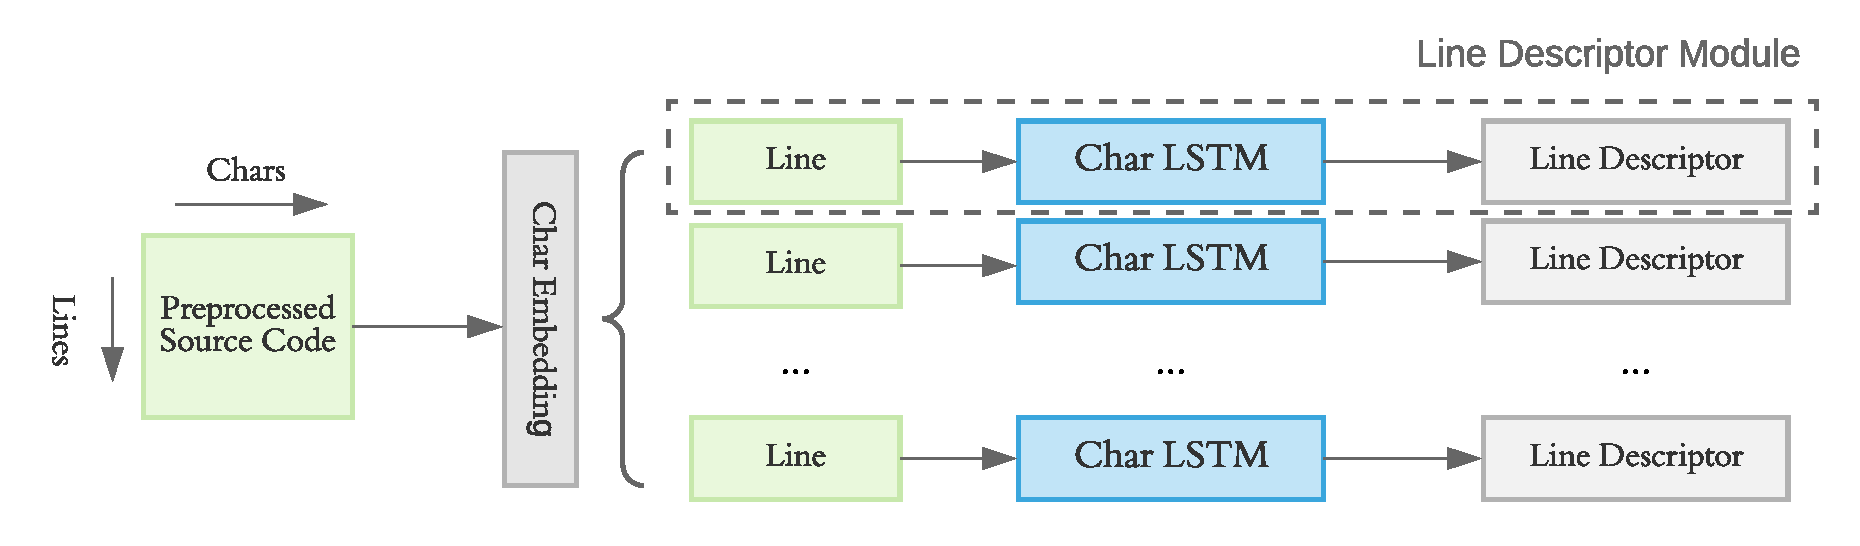
\includegraphics[width=\linewidth]{imgs/lstm_char_level.pdf}
		\subcaption{Char embedding layer and line descriptor module}\label{fig:lstm_architecture:a}
	\end{subfigure}%
	\\
	\begin{subfigure}[t]{\textwidth}
		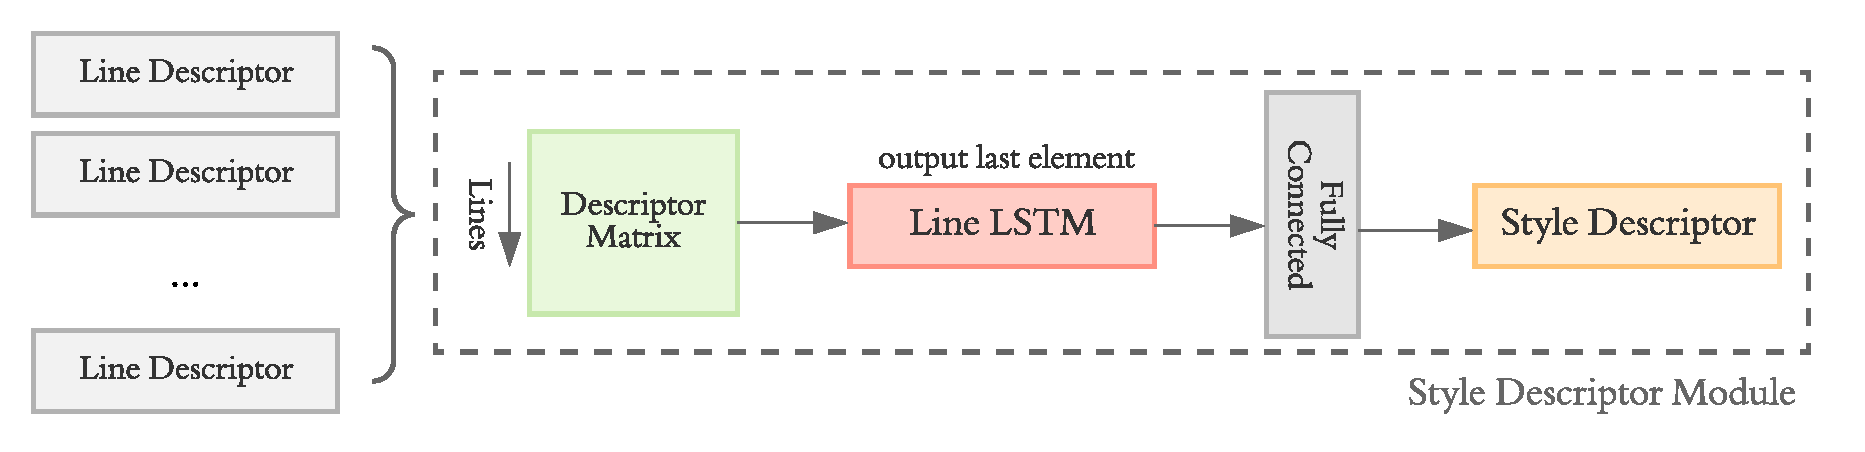
\includegraphics[width=\linewidth]{imgs/lstm_line_level.pdf}
		\subcaption{Style descriptor module}\label{fig:lstm_architecture:b}
	\end{subfigure}%
	\caption{The architecture of the LSTM-based model.}
	\label{fig:lstm_architecture}
\end{figure}

Our proposed architecture can be split in three parts: the char embedding layer, the line descriptor module (Fig. \ref{fig:lstm_architecture:a}) and the style descriptor module (Fig. \ref{fig:lstm_architecture:b}).

\subparagraph*{Char Embedding Layer}

Neural networks can't handle discrete types -- like chars -- naturally. As such, we need to map the alphabet $\Sigma$ of source codes to real-valued vectors. We could simply convert each char to a $|\Sigma|$-dimensional one-hot vector. As opposed to arbitrarily defining a mapping, we could also let the network learn it. 

The char embedding layer is responsible for learning an embedding $f_c(x) \in \mathbb{R}^{d_c}$ that maps chars to $d_c$-dimensional vectors. Thus, each char in the source code is converted to a real-valued vector. Hereon, we will simply refer to the char embeddings as chars.
% TODO: add referencia pro embedding do keras

\subparagraph*{Line Descriptor Module} 

This module is responsible for learning an embedding $f_l(x) \in \mathbb{R}^{d_l}$ that maps lines of code to $d_l$-dimensional descriptors. Each line of the source code is fed -- char by char -- to the same char-level bidirectional LSTM with (...) hidden units.

\subparagraph*{Style Descriptor Module}

The line descriptors generated by the line descriptor module are stacked back into a descriptor matrix. This module is responsible for learning an embedding $f_s(x) \in \mathbb{R}^d$ that maps descriptor matrices to $d$-dimensional style descriptors. Thus, the whole descriptor matrix is fed -- line by line -- to a line-level bidirectional LSTM, passed through a fully-connected layer and normalized to lie on the $d$-sphere. The resulting descriptor is the desired style descriptor.

We believe this architecture encourages the network to learn in a divide-and-conquer manner, by learning the individual features of each line and how to combine them into a single descriptor. The hyperparameter values chosen through the validation phase are given in Table \ref{tab:lstm_hyper}.

\begin{table}[htbp]
	\centering
	\begin{tabular}{|c|l|}
		\hline
		\textbf{Parameter}           & \multicolumn{1}{c|}{\textbf{\#}} \\ \hline
		$d_c$, char embedding size   & (...)                            \\ \hline
		$d_l$, line descriptor size  & (...)                            \\ \hline
		$d_s$, style descriptor size & (...)                            \\ \hline
		char-level LSTM hidden units & (...)                            \\ \hline
		line-level LSTM hidden units & (...)                            \\ \hline
		fully-connected layer units  & (...)                            \\ \hline
	\end{tabular}
	\caption{Values for the hyperparameters of the LSTM-based model.}
	\label{tab:lstm_hyper}
\end{table}

\subsection{Optimization}\label{sec:optimization}
%TODO: optimization preamble

\subsubsection{Softmax Cross-Entropy Loss}\label{sec:softmax}

The softmax function is commonly used in multi-class classification problems. In a $d$-class scenario, let $f(x) \in \mathbb{R}^d$ be the output of our neural network for a sample $x$. ...

\begin{equation}
q(i) = \frac{e^{f(x)_i}}{\sum_j e^{f(x)_j}} \,.
\end{equation}

$q(i)$ assume values ranging from 0 to 1, and $\sum_i a_i = 1$. Therefore, we can reinterpret $q(i)$ as the estimation of probability the sample $x$ belongs to class $i$. The softmax cross-entropy loss is given as

\begin{equation}
\mathcal{L} = -\sum_{i=1}^d p(x, i) \log q(i) \,,
\end{equation}

where $p(x, i)$ is the actual probability the sample $x$ is from class $i$ (usually a one-hot vector). Thus, by minimizing $\mathcal{L}$, we minimize the cross-entropy between the probability distribution $p$ and an estimated distribution $q$.

Although softmax cross-entropy loss is a very powerful tool, it does not naturally account for the fact that the number of classes may be unknown. Although there are techniques to apply softmax in these scenarios \cite{softmax_trick1,softmax_trick2}, there are other optimization methods designed for such cases. Therefore, we restrict ourselves to use this method only when the number of classes is known.

\subsubsection{Triplet Loss}\label{sec:triplet}

\citeonline{facenet} introduced triplet loss for training embedding networks. In their work, the loss function is used in conjunction with a novel triplet mining algorithm to train an embedding network that maps images to descriptors. These descriptors are then used to solve face recognition. Triplet loss works in scenarios where the number of classes is unknown. As such, it is well-suited for deciding if two pieces of code are of the same person, even if they are unknown to the system.

The embedding is represented by $f(x) \in \mathbb{R}^d$. Additionally, we constrain this embedding to the boundary of a $d$-sphere, \textit{i.e.} $\norm{f(x)}_2 = 1$.

Let $a, p, n$ (stand for anchor, positive and negative, respectively) be a triplet from the training set such that $a$ and $p$ have the same label (positive pair), but $a$ and $n$ have different labels (negative pair). Also, let $\mathcal{T}$ be the set of all possible said triplets.. Then, triplet loss is defined as

\begin{equation}\label{eq:triplet}
\mathcal{L} = \sum_{(a, p, n) \in \mathcal{T}} %
%\Bigl[\ \norm{f(a) - f(p)}_2 - \norm{f(a) - f(n)}_2 + \alpha \ \Bigr] _+\,,
\max\Bigl(\ \norm{f(a) - f(p)}_2 - \norm{f(a) - f(n)}_2 + \alpha,\ 0\Bigr)\,,
\end{equation}

where $\alpha$ is a margin that is enforced between positive and negative pairs. If $\mathcal{L} = 0$, then for every triplet $(a, p, n) \in T$, it must be true that

\begin{equation}\label{eq:triplet_condition}
\norm{f(a) - f(p)}_2 + \alpha \leq \norm{f(a) - f(n)}_2 \,.
\end{equation}

When Eq. \ref{eq:triplet_condition} is fulfilled, the negative pair of a triplet will be at least as far as the positive pair plus a margin $\alpha$. Thus, by minimizing $\mathcal{L}$, we push the distance of positive pairs towards zero as we push the distance of negative pairs to be greater than the correspondent positive's by $\alpha$. The advantage of this formulation is that, even though all training samples of the same class will form a cluster, they are not required to collapse to a single point. Fig. \ref{fig:triplet} shows an hypothetical scenario of optimization.

Generating all triplets from $\mathcal{T}$ would consider many triplets that easily satistfy Eq. \ref{eq:triplet_condition}. This would cause the training to converge slowly, since those triplets would still be fed to the network, but would not contribute to loss minimization. Therefore, it is crucial to select triplets that do not satisfy this condition to keep improving the model. These are called \textit{hard} triplets.

% TODO: regenerate these pictures with correct casing and alpha
\begin{figure}[ht]
	\centering
	\begin{subfigure}[t]{0.25\textwidth}
		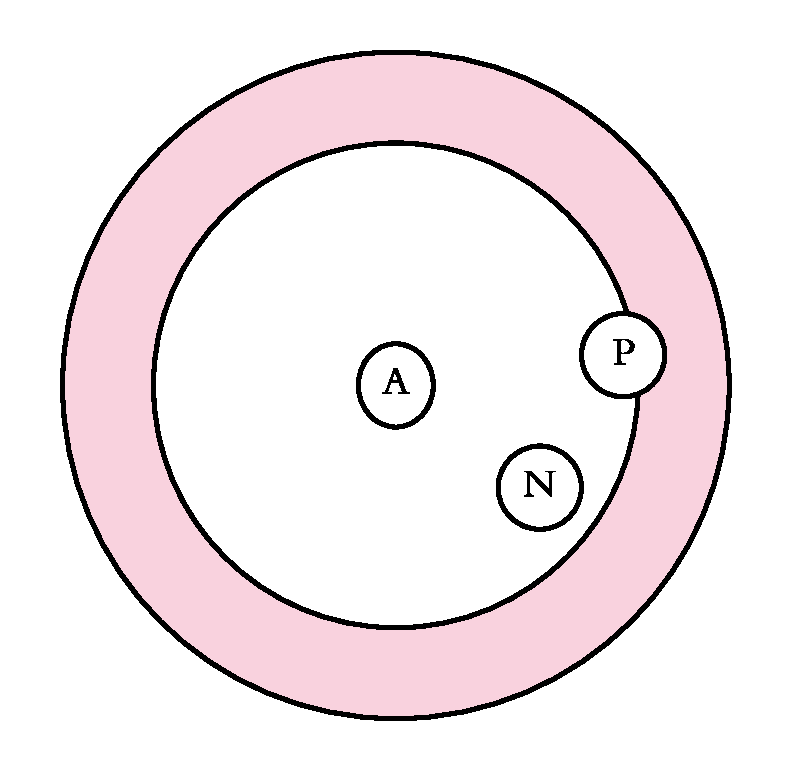
\includegraphics[width=\linewidth]{imgs/triplet_loss_before.pdf}
		\subcaption{}\label{fig:triplet:a}
	\end{subfigure}%
	\hspace{1cm}%
	\begin{subfigure}[t]{0.25\textwidth}
		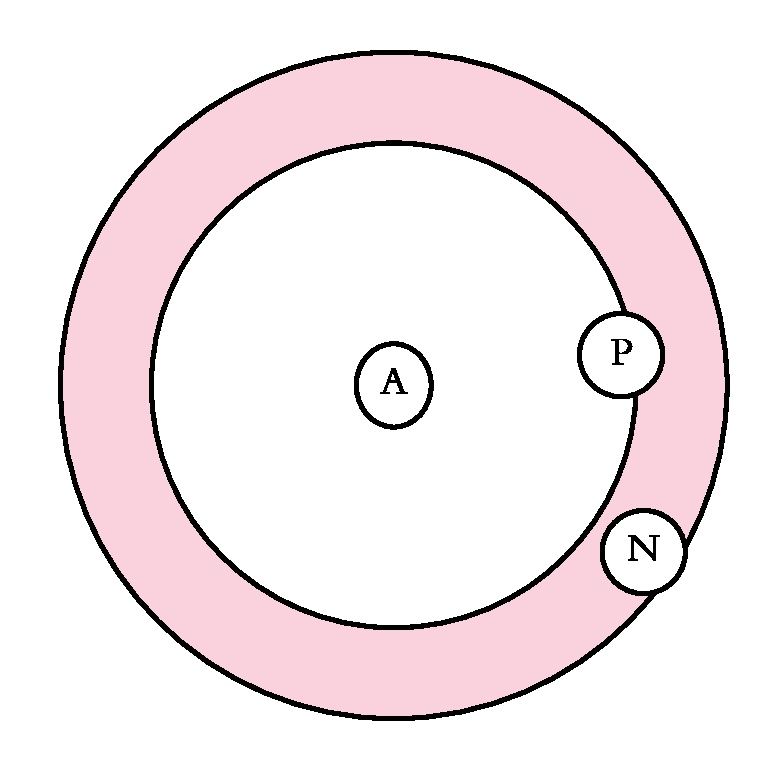
\includegraphics[width=\linewidth]{imgs/triplet_loss_during.pdf}
		\subcaption{}\label{fig:triplet:b}
	\end{subfigure}%
	\hspace{1cm}%
	\begin{subfigure}[t]{0.25\textwidth}
		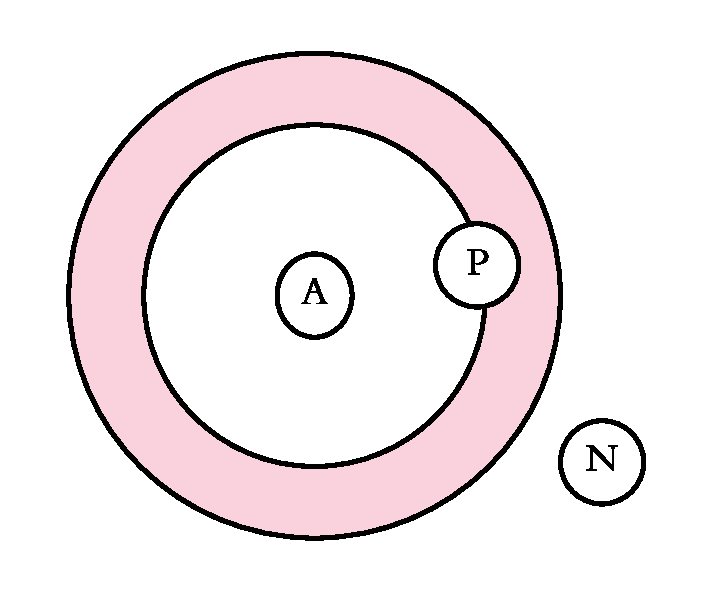
\includegraphics[width=\linewidth]{imgs/triplet_loss_after.pdf}
		\subcaption{}\label{fig:triplet:c}
	\end{subfigure}%
	\caption{The region in red represents the margin area beyond $p$ with diameter $\alpha$. Before loss optimization (\subref{fig:triplet:a}), the negative pair is closer than the positive. During loss optimization (\subref{fig:triplet:b}), the negative pair is pushed further than the positive, but $n$ is still in the margin area. After loss optimization (\subref{fig:triplet:c}), the positive pair is finally closer and $n$ is beyond the margin.}
	\label{fig:triplet}
\end{figure}

\subparagraph*{Online Semi-Hard Triplet Mining} One way to select hard triplets from the training set is to consider every sample as the anchor $a$. Then, select such $p$ that minimizes $\norm{f(a) - f(n)}_2$ and such $n$ that maximizes $\norm{f(a) - f(n)}_2$. This does not scale with the size of the training set. Moreover, it can cause outliers to dominate the selection process. 

\citeauthoronline{facenet} suggested the online semi-hard triplet mining method to tackle both problems. Instead of picking hard triplets from the whole training set, we pick them from the mini-batch. Also, their work suggests that prioritizing triplets such that negatives lie in the margin area (Fig. \ref{fig:triplet:b}) helps avoiding local minima early in the training. Such triplets are called \textit{semi-hard}.

Although in Chapter (...) we use softmax cross-entropy loss for comparison purposes, we mostly worked with triplet loss.  Therefore, our main optimization flow is pictured in Fig. \ref{fig:triplet_overall}.

\begin{figure}[ht]
	\centering
	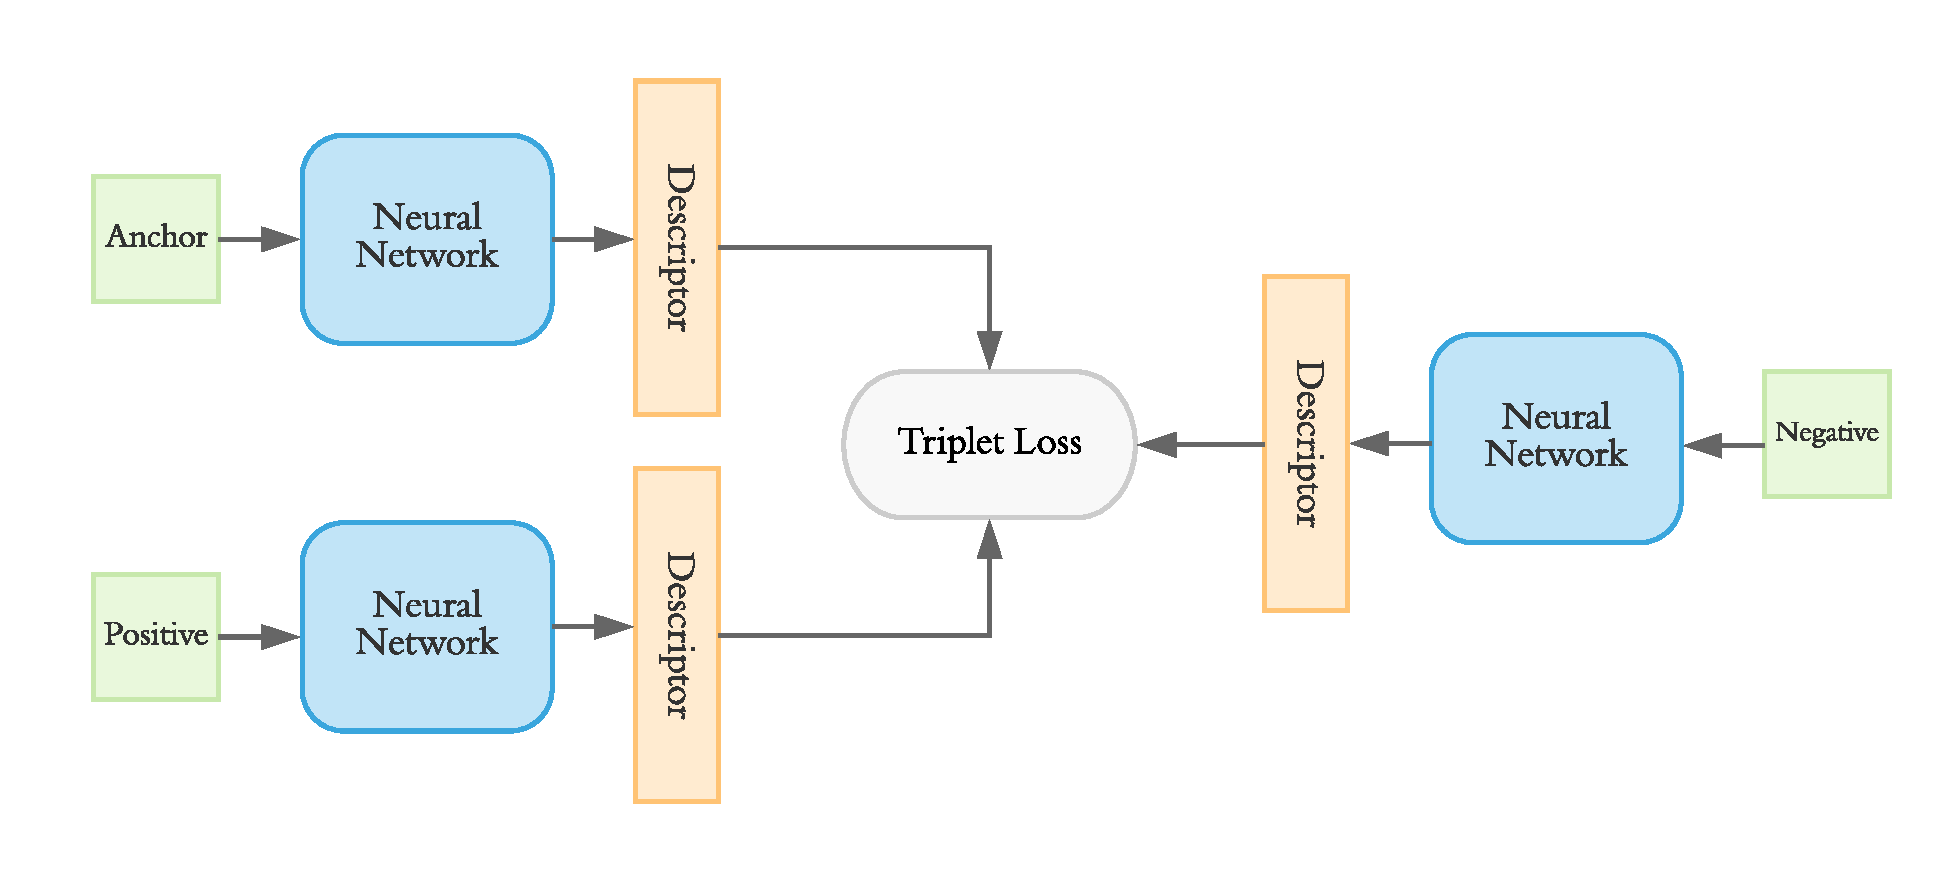
\includegraphics[width=\linewidth]{imgs/triplet_loss_architecture.pdf}
	\caption{Overview of style descriptor generation pipeline.}
	\label{fig:triplet_overall}
\end{figure}